
Se desea realizar un despliegue del proyecto, de forma que los modelos de predicción sean accesibles mediante una interfaz web. Especificamente, se plantea que cualquier usuario 
pueda seleccionar una de las estaciones de Grafcan, y a partir de la misma, que la aplicación web devuelva la predicción de alguna de las variables meteorológicas en las próximas horas. 
Se decide arbitrariamente acotar a la variable de temperatura y las próximas 3 horas.

Se realiza una interfaz web sencilla como front-end, y un back-end que maneje la carga de trabajo de predicción.

\section{Front-end}
Tras valorar distintas opciones, se elige React como framework para el front-end. Se decide por su facilidad de uso y la gran cantidad de librerías que existen para este.
Se emplea typescript para la codificación, al ser una alternativa más robusta a javascript, y que permite detectar errores de forma más sencilla.

Se crea una aplicación de una sola página (Single Page Application) que permite al usuario buscar y seleccionar una estación de Grafcan. Una vez seleccionada,
se envía una petición al back-end para obtener la predicción.

Para el desarrollo de la aplicación es necesario crear una serie de elementos denominados "componentes". Estos componentes son bloques de código que 
permiten crear una interfaz de usuario modular y reutilizable. En este caso, se crean, entre otros
\begin{itemize}
    \item \textbf{App}: Componente principal de la aplicación. Se encarga de gestionar el estado de la aplicación y de renderizar los demás componentes.
  
\end{itemize}


\section{Back-end}

\begin{figure}[H]
    \centering
    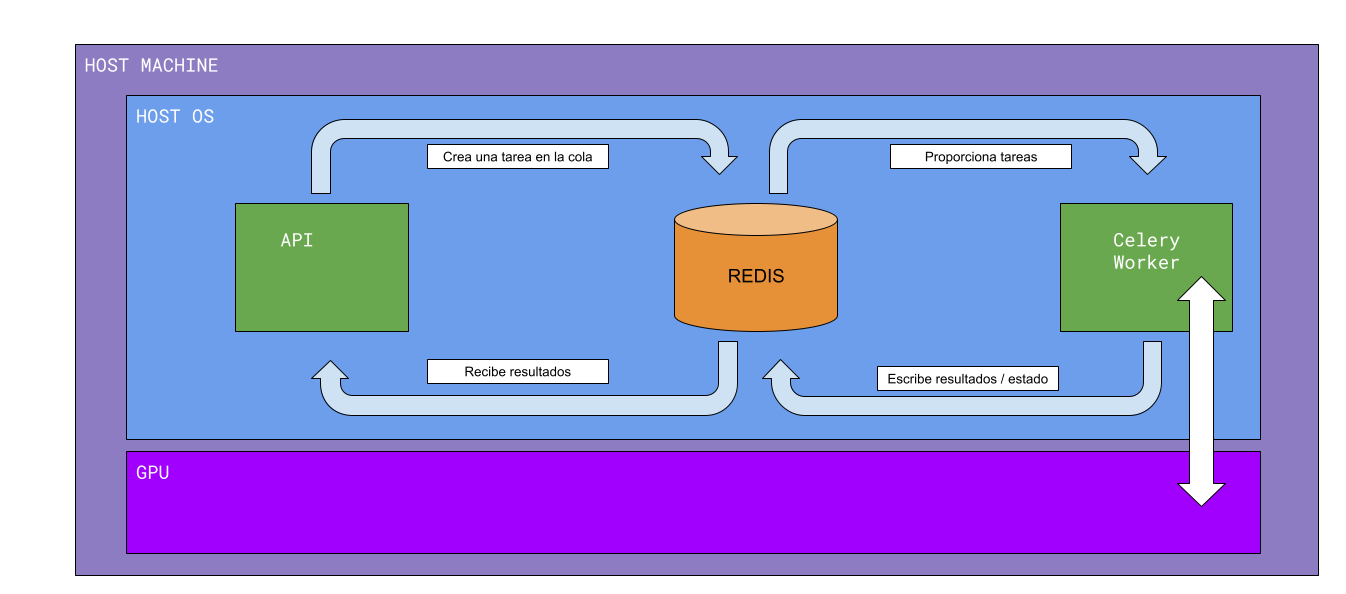
\includegraphics[width=0.9\textwidth]{images/esquema_despliegue.png}
    \caption{Esquema de la lógica del desplieuge}
    \label{deploy_scheme}
\end{figure}